%%%%%%%%%%%%%%%%%%%%%%%%%%%%%%%%%%%%%%%%%%%%%%%%%%%%%%%%%%%%%%%%%%%%%%%%%%%%
% AGUJournalTemplate.tex: this template file is for articles formatted with LaTeX
%
% This file includes commands and instructions
% given in the order necessary to produce a final output that will
% satisfy AGU requirements, including customized APA reference formatting.
%
% You may copy this file and give it your
% article name, and enter your text.
%
%
% Step 1: Set the \documentclass
%
%

%% To submit your paper:
\documentclass[draft]{agujournal2019}
\usepackage{url} %this package should fix any errors with URLs in refs.
\usepackage{lineno}
\usepackage[inline]{trackchanges} %for better track changes. finalnew option will compile document with changes incorporated.
\usepackage{soul}
\usepackage{caption}

\linenumbers
%%%%%%%
% As of 2018 we recommend use of the TrackChanges package to mark revisions.
% The trackchanges package adds five new LaTeX commands:
%
%  \note[editor]{The note}
%  \annote[editor]{Text to annotate}{The note}
%  \add[editor]{Text to add}
%  \remove[editor]{Text to remove}
%  \change[editor]{Text to remove}{Text to add}
%
% complete documentation is here: http://trackchanges.sourceforge.net/
%%%%%%%

\draftfalse

%% Enter journal name below.
%% Choose from this list of Journals:
%
% JGR: Atmospheres
% JGR: Biogeosciences
% JGR: Earth Surface
% JGR: Oceans
% JGR: Planets
% JGR: Solid Earth
% JGR: Space Physics
% Global Biogeochemical Cycles
% Geophysical Research Letters
% Paleoceanography and Paleoclimatology
% Radio Science
% Reviews of Geophysics
% Tectonics
% Space Weather
% Water Resources Research
% Geochemistry, Geophysics, Geosystems
% Journal of Advances in Modeling Earth Systems (JAMES)
% Earth's Future
% Earth and Space Science
% Geohealth
%
% ie, \journalname{Water Resources Research}

\journalname{Geophysical Review Letters}


\newcommand{\markred}[1]{\textcolor{red}{#1}}
%\newcommand{\markcyan}[1]{\textcolor{cyan}{#1}}
\newcommand{\markblue}[1]{\textcolor{blue}{#1}}
%\newcommand{\markgreen}[1]{\textcolor{magenta}{#1}}


\begin{document}

%% ------------------------------------------------------------------------ %%
%  Title
%
% (A title should be specific, informative, and brief. Use
% abbreviations only if they are defined in the abstract. Titles that
% start with general keywords then specific terms are optimized in
% searches)
%
%% ------------------------------------------------------------------------ %%

% Example: \title{This is a test title}

\title{Measuring and modeling local hydraulic resistance in heterogeneous porous media}

%% ------------------------------------------------------------------------ %%
%
%  AUTHORS AND AFFILIATIONS
%
%% ------------------------------------------------------------------------ %%

% Authors are individuals who have significantly contributed to the
% research and preparation of the article. Group authors are allowed, if
% each author in the group is separately identified in an appendix.)

% List authors by first name or initial followed by last name and
% separated by commas. Use \affil{} to number affiliations, and
% \thanks{} for author notes.
% Additional author notes should be indicated with \thanks{} (for
% example, for current addresses).

% Example: \authors{A. B. Author\affil{1}\thanks{Current address, Antartica}, B. C. Author\affil{2,3}, and D. E.
% Author\affil{3,4}\thanks{Also funded by Monsanto.}}

\authors{Quirine Krol \affil{1}, Itzhak Fouxon \affil{1,2}, Pascal Corso \affil{1}, Markus Holzner \affil{1,2,3,4}}



\affiliation{1}{ETH Zurich, Stefano Franscini-Platz 5, 8093 Zurich, Switzerland}
\affiliation{2}{Department of Computational Science and Engineering, Yonsei University, Seoul 120-749, South Korea}
\affiliation{3}{Swiss Federal Institute for Water Science and Technology EAWAG}
\affiliation{4}{Swiss Federal Institute for Forest, Snow and Landscape Research WSL}


%(repeat as many times as is necessary)

%% Corresponding Author:
% Corresponding author mailing address and e-mail address:

% (include name and email addresses of the corresponding author.  More
% than one corresponding author is allowed in this LaTeX file and for
% publication; but only one corresponding author is allowed in our
% editorial system.)

% Example: \correspondingauthor{First and Last Name}{email@address.edu}

\correspondingauthor{Markus Holzner}{holzner@wsl.ch}

%% Keypoints, final entry on title page.

%  List up to three key points (at least one is required)
%  Key Points summarize the main points and conclusions of the article
%  Each must be 140 characters or fewer with no special characters or punctuation and must be complete sentences

% Example:
% \begin{keypoints}
% \item	List up to three key points (at least one is required)
% \item	Key Points summarize the main points and conclusions of the article
% \item	Each must be 140 characters or fewer with no special characters or punctuation and must be complete sentences
% \end{keypoints}

\begin{keypoints}
\item We introduce a new definition for individual pores in heterogeneous porous media based on iso-pressure surfaces.
\item We employ direct numerical simulations to measure the local hydraulic conductivity. 
\item We model the local hydraulic resistance of a pore based on local sphericity and channelization of iso-pressure surfaces. 
\end{keypoints}

%% ------------------------------------------------------------------------ %%
%
%  ABSTRACT and PLAIN LANGUAGE SUMMARY
%
% A good Abstract will begin with a short description of the problem
% being addressed, briefly describe the new data or analyses, then
% briefly states the main conclusion(s) and how they are supported and
% uncertainties.

% The Plain Language Summary should be written for a broad audience,
% including journalists and the science-interested public, that will not have 
% a background in your field.
%
% A Plain Language Summary is required in GRL, JGR: Planets, JGR: Biogeosciences,
% JGR: Oceans, G-Cubed, Reviews of Geophysics, and JAMES.
% see http://sharingscience.agu.org/creating-plain-language-summary/)
%
%% ------------------------------------------------------------------------ %%

%% \begin{abstract} starts the second page

\begin{abstract}
[ Resolving local velocities for laminar flow in porous media is essential to transport processes. Using direct numerical simulations to solve the Navier-Stokes equations is computationally costly for statistical representative volumes. Pore network models allow for much faster solutions and resolve much larger domains. However, the pore network architecture and constitutive model for the hydraulic resistance heavily influence the permeability and the quality of local velocity predictions. Here, we investigate the validity of a commonly used constitutive law. We start by generating three three-dimensional artificial geometries representing porous media. In this way we can control the geometrical parameters, such as the porosity and the averaged interface area. As a benchmark, we use high fidelity numerical simulations of the Navier-Stokes equations to resolve the pressure and velocity field for laminar flow in the pore-space of the artificial geometries. We propose a new definition for pores based on iso-pressure surfaces and topology changes that enables us to measure the local hydraulic resistance. We show that it can be over-estimated up to two orders of magnitude. We propose a new constitutive model that is based on the geometry of iso-pressure surfaces. This model shows that the sphericity of iso-pressure surfaces is key to predict the local hydraulic resistances of heterogeneous porous media more reliable. The distributions of local resistances and effective pore lengths show an interesting pathway to new statistical network representations of laminar flow in porous media.]
\end{abstract}

\section*{Plain Language Summary}
[ enter your Plain Language Summary here or delete this section]


%% ------------------------------------------------------------------------ %%
%
%  TEXT
%
%% ------------------------------------------------------------------------ %%

%%% Suggested section heads:
\section{Introduction}

Porous media flow is important for a wide range of applications in nature and technology, spanning from groundwater remediation and oil recovery to packed bed reactors and particle filters. In these flows, the highly complex and three-dimensional pore geometries give rise to complicated pore velocity fields that form the backbone for transport, mixing and chemical reaction processes. Detailed knowledge of these velocity fields is important for the modelling of effective parameters, most notably the permeability and the prediction of transport in porous media \cite{bear_dynamics_1972,scheidegger_physics_1974}. Despite its importance and extensive research, however, the relation between geometrical features of porous media and the resulting flow is still not fully understood.
Given that detailed knowledge of geometrical features of porous media is often unavailable, the classical flow modeling approach has been to represent the porous medium as a lattice of circular tubes that represent the pore network \cite{scheidegger_physics_1974}. The flow in the tubes is assumed uniform and the velocity profile parabolic. While this is a rather crude approximation of the real geometry and flow behaviors, it has provided useful predictions for flow and transport. Early studies have modelled velocity distributions \cite{haring_statistical_1970}, permeability \cite{fatt_network_1956,katz_quantitative_1986} and particle dispersion \cite{saffman_theory_1959} based on bulk statistics of the medium geometry such as pore size distributions. These early studies have spurred many subsequent works on statistical pore scale models (e.g. \cite{dullien_single_1975,kutsovsky_nmr_1996,maier_simulation_1999,siena_relationship_2014,de_anna_prediction_2017}. The second class of models that hinges on the simplified lattice representation of porous media are the so-called pore network models \cite{thompson_modeling_1997}. For both classes of models, the simplified modelling of local resistivity based on Hagen-Poisseuille is a central element.
Many authors tried to relate the statistics of pore velocity to statistics of pore geometry represented by e.g. the local pore radius, the connectivity between pores etc. For example, one of the simplest models is the so-called \emph{capillary bundle} model, in which the porous medium is conceptualized as a parallel arrangement of capillaries with given pore sizes \citeA{scheidegger_physics_1974}. Extensions of this model include parallel arrangements of wavy tubes \citeA{le_borgne_effective_2011}. These simple models are not appropriate for complex porous media, for which the network aspect is important. That is, in general, the connectivity between pores cannot be neglected and the concept of the linear pore breaks down. An ad-hoc model that conceptualizes flow in porous media as a system of serial and parallel pore arrangements can be found in \cite{holzner_intermittent_2015}. \cite{siena_relationship_2014} statistically related velocity distributions to pore size distributions of statistically generated 3D porous media. Based on direct numerical simulations in 2D porous media composed of disks, \cite{de_anna_prediction_2017} showed that the low velocity tail of the pore velocity distribution is governed by local pore radius. This is a notable result as it suggests that the slow flow velocities are not strongly dependent on the connectivity between pores. \cite{alim_local_2017} showed that pore velocity distributions are governed by local correlations of pore radii that organize flux ratios at pore junctions. As mentioned, the statistical models in these works are based on the concept that local velocity profiles are parabolic. Some recent papers provided qualitative examples comparing pore velocity profiles to a parabola that suggest the assumption may be reasonable \citeA{de_anna_prediction_2017,dentz_mechanisms_2018}. In the present paper, we present a rigorous assessment of local hydraulic resitances in three-dimensional pore geometries based on statistically generated 3D porous media.
With the advent of experimental techniques like microcomputed tomography there is now access to impressive details of three dimensional porous media architectures. Even though today’s computing facilities make it possible to solve flow and transport with unprecedented accuracy in these complex geometries using direct numerical simulations, this approach is only feasible in small domains. Simple models that reduce the full complexity of real porous media are still needed. A lattice representation is the standard approach in so-called pore network models in which a Kirchhoff-type system of equations is solved to model single or multiphase porous medium flows \citeA{thompson_modeling_1997}. The lattice is usually constructed based on data from experimental pore scale characterization measurements, e.g. imaging or mercury intrusion porosimetry. These pore network models are a valuable tool for understanding meso-scale phenomena, linking single pore processes and continuum porous media used in engineering \citeA{xiong_review_2016}. Besides a sound network construction approach that mimics the real media, another critical aspect for the accuracy of modeling is the representation of local resistivity in the pores. In this paper, we perform Direct Numerical Simulations (DNS) that solve the Navier-Stokes equations in heterogeneous porous media. The boundary conditions are chosen such that Re number is chosen within the Stokes regime $Re\ll1$. These simulations enables us to know the locally the velocity $\mathbf{u}$ and the local pressure field $p$. We propose a new definition of local pores for which we can measure the local pressure drop and the internal hydraulic resistance of the porous media. In this manner we can test how well the Hagen-Poiseuille 



\section{Theoretical Background}
\subsection{Static Navier stokes equations in porous media}
We assume that for low Reynolds number, incompressible flow in a porous media, the local flow can be described by the Navier-Stokes equations. 
\begin{equation}
	\mathbf{\nabla} p = - \mu\mathbf{\nabla}^2 \mathbf{u}\,,\,\mathbf{\nabla}\cdot\mathbf{u}=0\label{eq:stokes_local}
	\end{equation}
with pressure $p$ and velocity $\mathbf{u}$ and dynamic viscosity $\nu$. 
For a volume $V$ in a porous media, enclosed by surface $\partial V$ given by two isopressure surfaces $S_{p_1}$ and $S_{p_2}$ and a remaining a porous media domain $\Gamma$, we can write down the integral form of the Navier-Stokes equations


\begin{equation}
\int_V \left(\mathbf{u}\cdot\mathbf{\nabla} p-\mu \mathbf{u}\cdot\mathbf{\nabla}^2 \mathbf{u}\right) dV 
= \int_{\partial V}  p\,\mathbf{u}\cdot\mathbf{n}\,dS+\mu \int_{\partial V} \mathbf{u} (\mathbf{\nabla} \mathbf{u})\cdot\mathbf{n}\,dS-\mu \int_{V} (\mathbf{\nabla}\, \mathbf{u})^2 dV=0 \label{eq:stokes_dissipation}
\end{equation}

Given that at the porous media boundary domain $\Gamma$ we have a no-slip condition $\mathbf{u}=0$ we can write \markred{check signs}

\begin{equation}
	Q \Delta p = -\mu\int_{S_{p_1}+S_{p_2}} \mathbf{u} (\mathbf{\nabla} \mathbf{u})\cdot\mathbf{n}\,dS -\mu \int_V (\mathbf{\nabla}\, \mathbf{u})^2 dV, \label{eq:pressuredrop}
\end{equation}


with the total flux defined by 

\begin{equation}
	Q=\int \mathbf{u}\cdot\mathbf{n}\, dS.
\end{equation}




\subsection{Pore identification}

\begin{centering}
\begin{figure}[t!]\label{fig:isop_surfaces}
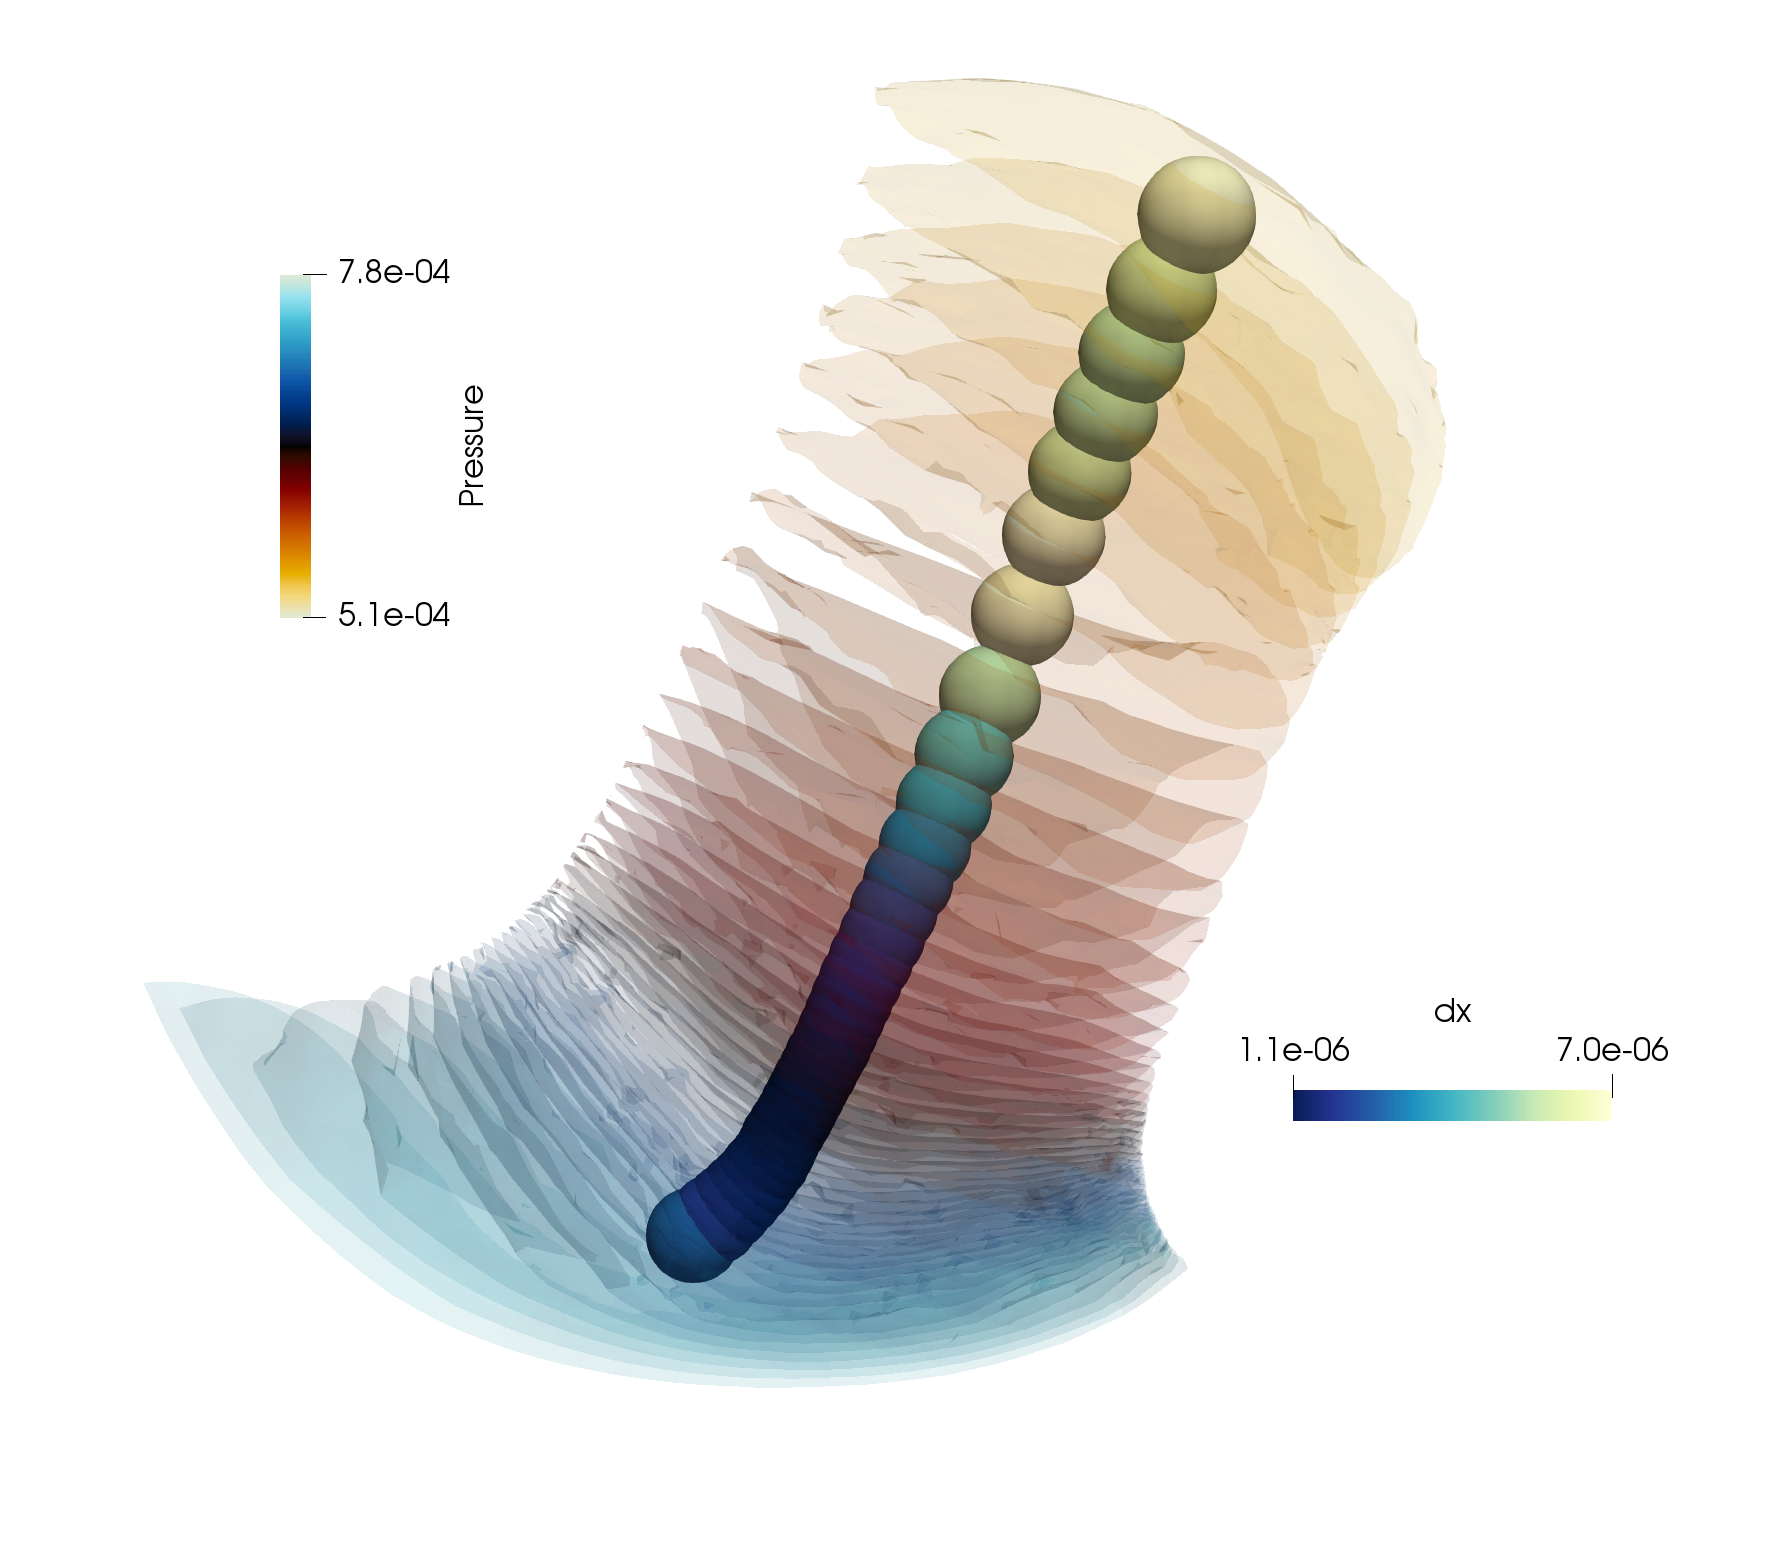
\includegraphics[height=5cm]{figures/example_pore.png}~~~~
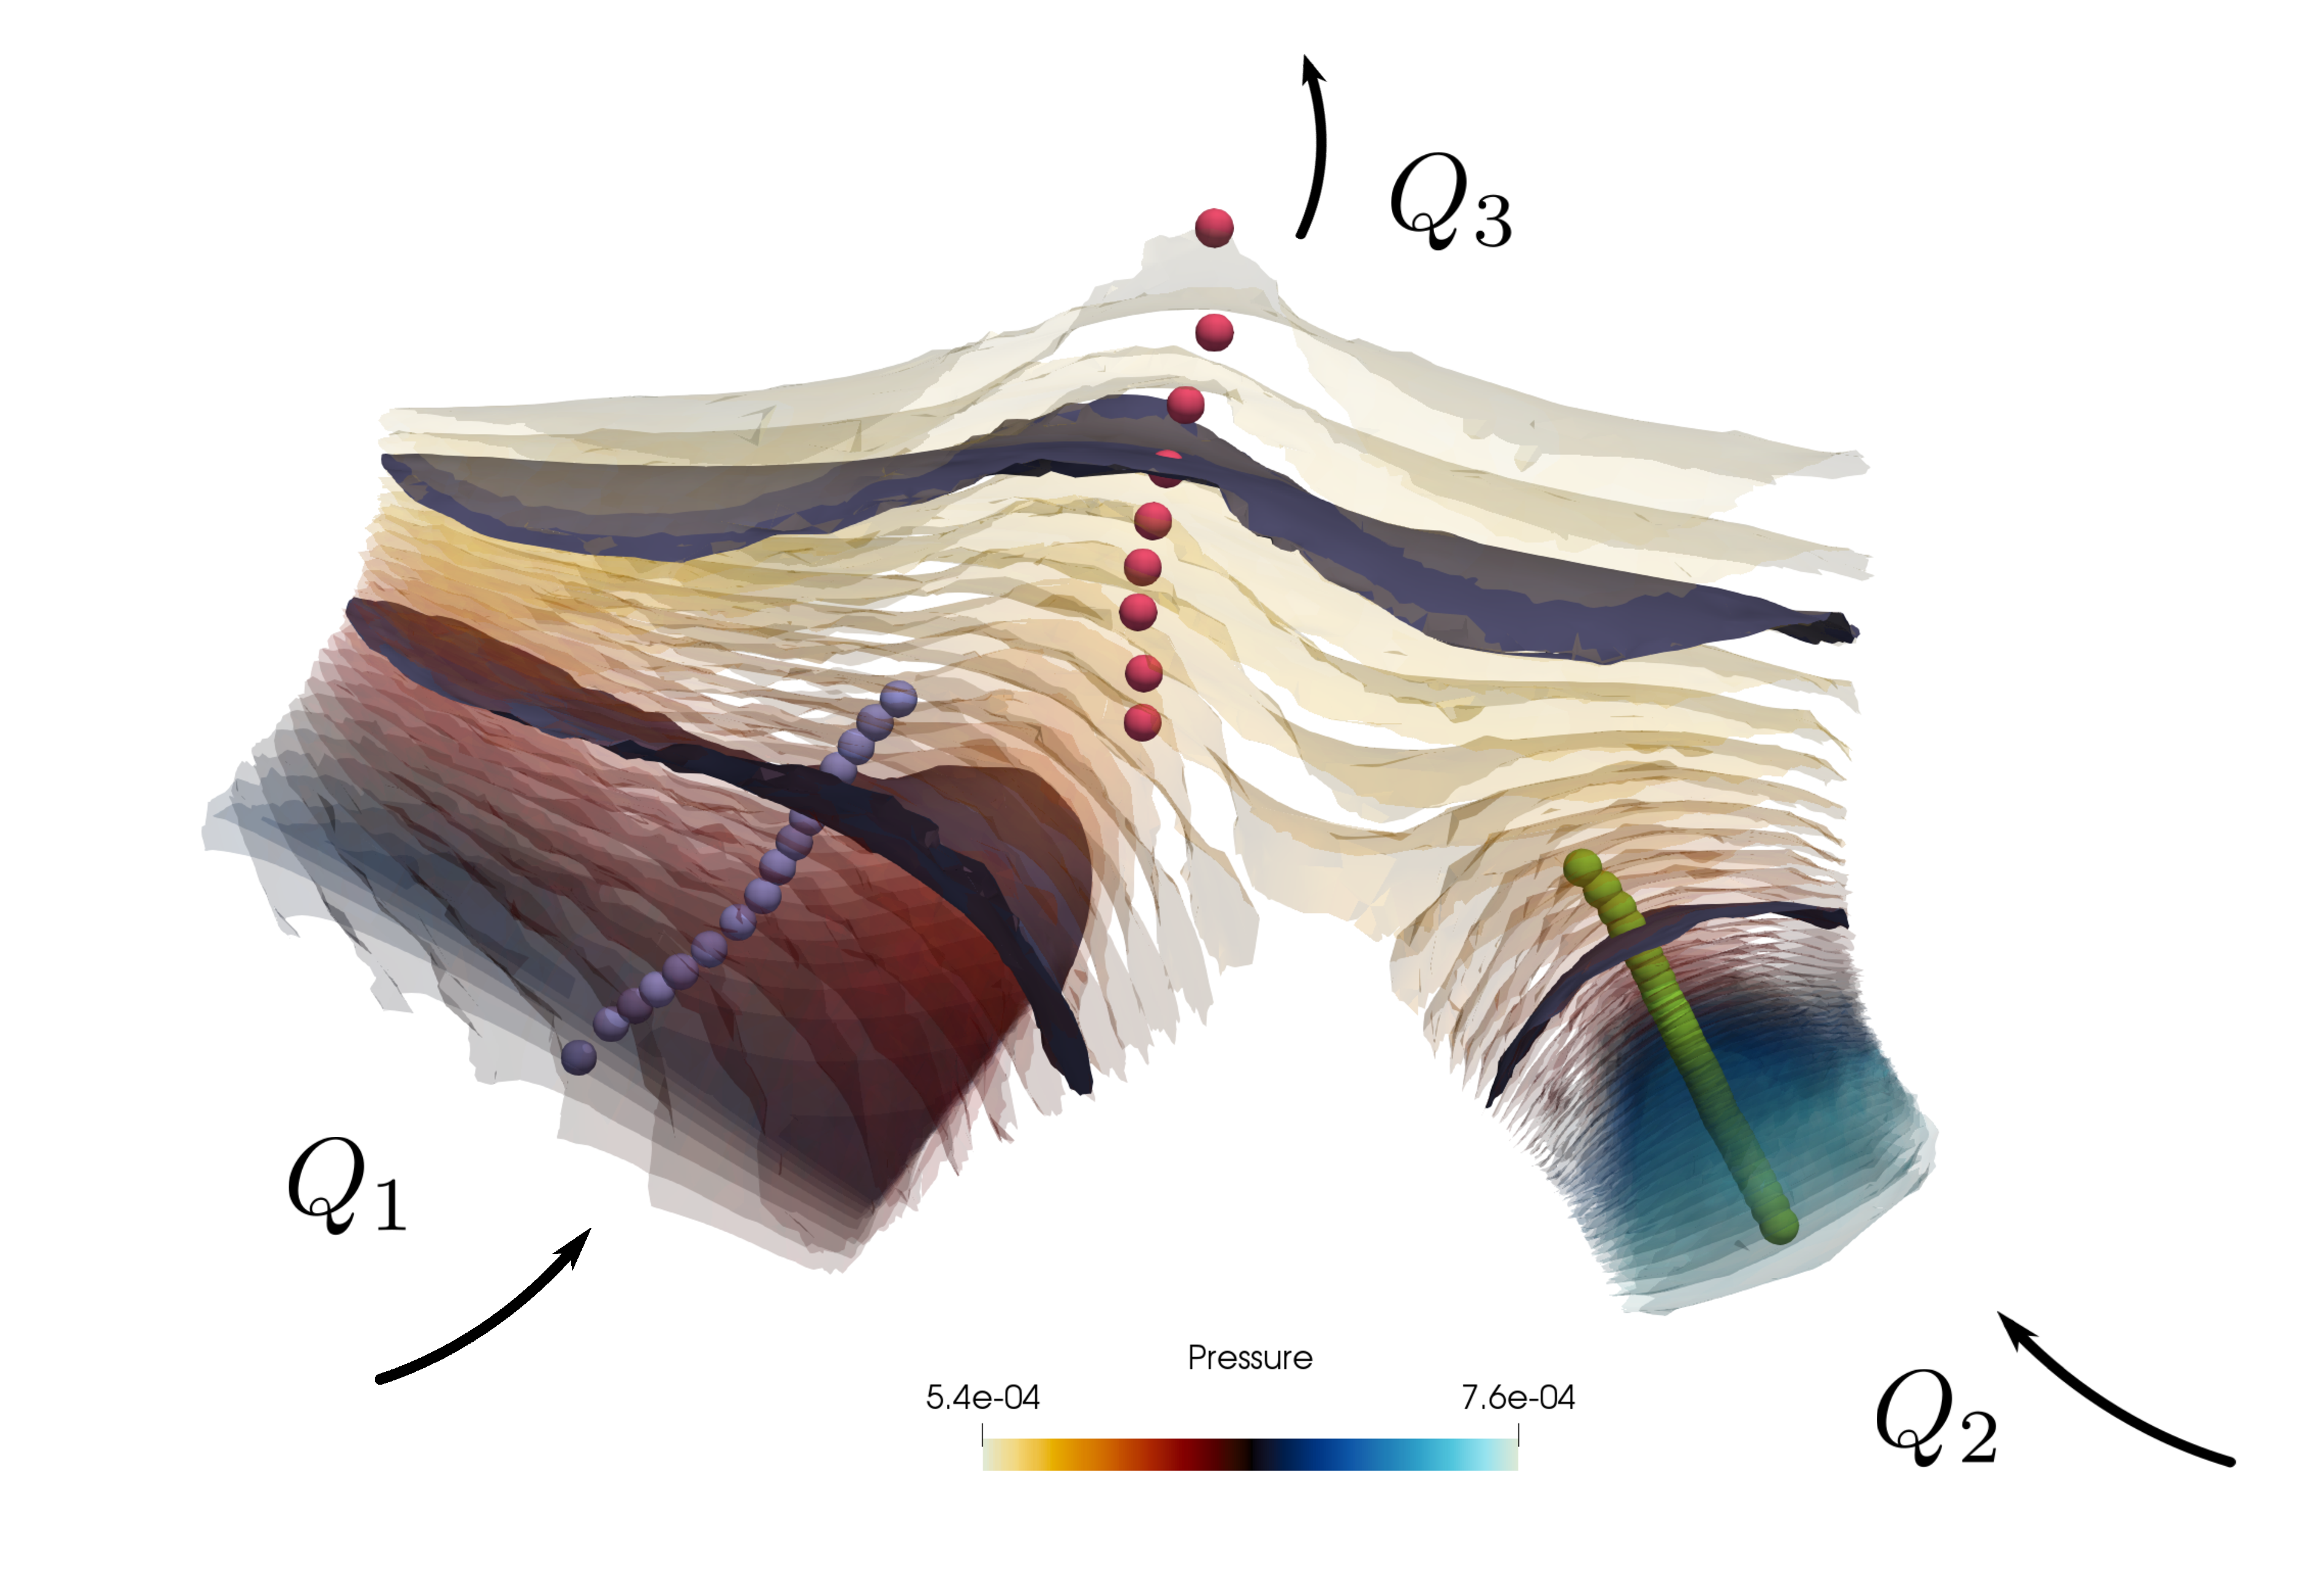
\includegraphics[height=5cm]{figures/merging_pores.eps}
\caption{Left: A visualization of a collection of consecutive iso-pressure surfaces comprising one pore, including the average coordinates of the iso-pressure surfaces indicated by the spheres. The color code of the spheres is given by the distance between the average coordinates between two consecutive iso-pressure surfaces. Right: A visualization of a junction of three pores for which the total flux is conserved $\sum_{i=1}^3 Q_i = 0$. This visualization is based on a subset of the DNS results of porous media \#2}
\end{figure}
\end{centering}
Here we introduce the notion of disconnected iso-pressure surfaces $\mathcal{S}_i(p)$ for a given pressure value $p$.
It is useful to observe that this consideration works for any fluid tube bounded by iso-pressure surfaces and iso-pressure surface of velocity magnitude at which velocity is (approximately) zero. Considering completely saturated conditions the boundary terms of Eq.~\ref{eq:stokes_dissipation} will be drop when multiple pores are added (meaning $\mathbf{n}\rightarrow -\mathbf{n}$). Therefore Eq.~\ref{eq:stokes_dissipation} intrinsically will only evaluate
\begin{equation}
Q \Delta p=\mu\int (\nabla \mathbf{u})^2 dV,\label{eq:pore_based_energy_dissipation}
\end{equation}

When we consider a decomposition of the velocity vector  $\mathbf{u} = u_p \mathbf{\hat{p}} + u_r \mathbf{\hat{r}}$ with $\mathbf{\hat{p}} =\mathbf{ \nabla}p/|\mathbf{ \nabla}p|$. For HP flow $\mathbf{u}$ is parallel to the pressure gradient, for which in simple geometries exact solutions can be derived. In the following we will assume that the most important contributions to the viscous dissipation tensor $\nabla_i u_j$ is given by the assumption that $\mathbf{\nabla}_i u_r \ll \mathbf{\nabla}_i u_p $. This assumption has been tested in the SI for the porous media that we have used below. This leads to 

\begin{equation}
\left|\nabla_i u_j\right|^2 \approx  \left|\nabla_r u_p\right|^2 + \left|\nabla_p u_p\right|^2 .\label{eq:reduced_dissipation_tensor}
\end{equation}

Here the first term is much more important since the velocity-velocity correlation length in the longitudinal direction is usually much larger than the average pore size. When we consider viscous dissipation of an infinitesimal enclosed volume $dV$ defined by $\mathcal{S}_i,\mathcal{S}_{i+1}$ and their respective areas $A_i, A_{i+1}$, separated by average distance $dx$ we can estimate the first term of Eq.~\ref{eq:reduced_dissipation_tensor} analogous as shown in \cite{mortensen_reexamination_2005} with
\begin{equation}
	\left|\nabla_r u_p\right|^2 =8\pi\mu \left(\alpha_0+\alpha_1\,\gamma^{-2}\right)\frac{ Q^2}{A^3}~~~ \rm{with}~~~ ,\label{eq:tau_1}
\end{equation}
with sphericity parameter $\gamma^{-1} = \mathcal{L}/\sqrt{ 4\pi A(p)}$ with perimeter $\mathcal{L} = \int_{\partial \mathcal{S}_i}dl$. The sphericity parameter is inversely related to the compactness factor $\gamma^{-2}\sim \mathcal{C}$ in \cite{mortensen_reexamination_2005}. The coefficient $a$ and $b$ can be calculated for simple shapes of the iso-pressure surfaces, such as squares, triangles, or a perturbation of a sphere by spherical harmonics \citeA{mortensen_reexamination_2005}. For heterogeneous media the class of shapes are generally unknown. For the second, longitudinal term, we can assume that the total flux $Q$ remains constant for $p\rightarrow p+dp$, and the change of velocity is caused by a change in cross-sectional area $A_i$, or in other words, the channelization of the pore 
\begin{equation}
	\left|\nabla_p u_p\right|^2 = \alpha_2  \frac{Q^2}{A^4}\left|\frac{\partial A}{\partial x }\right|^2,\label{eq:tau_2}
\end{equation}
with unknown $\alpha_2$. When we assume that for infinitesimal pressure differce $dp$, no topological changes (no junctions) of the isopressure surfaces take place, we can write $dV = A dl_{\rm{eff}}$, and we can combine the two expressions Eq.(\ref{eq:tau_1}) and Eq.(\ref{eq:tau_2}) into

\begin{equation}
	dp = 8\pi \mu \frac{Q(p)}{A(p)^2} f\left(\alpha_i,\mathcal{S}(p) \right) dx= 8 \pi \mu\frac{Q}{A^2}\left(\alpha_0+\alpha_1\gamma^{-2} + \alpha_2 \frac{1}{A}\left|\frac{\partial A}{\partial x}\right|^2\right)\,dx\label{eq:infi_dp}
\end{equation}
This expression is consistent with the Hagen-Poiseuille equation for pipe geometries $f(\alpha_i)\rightarrow 1$, and the local infinitesimal pressure gradient is given by 

\begin{equation}
		\frac{\partial p}{\partial x} = 8 \pi \mu\frac{Q}{A^2}, \label{eq:HP}
\end{equation}
Hereafter referred to as the HP-model. As long as there are no junctions Eq.(\ref{eq:infi_dp}) can be integrated. The total pressure gradient along a full pore is then given by

\begin{equation}
	\frac{\Delta p}{L_{\rm{eff}}} =  Q \frac{1}{L_{\rm{eff}}}\int^{L_{\rm{eff}}}_{0}\frac{1}{A^2}f\left(\alpha_i,\mathcal{S}(p)\right)\,dx
\end{equation}

with 
\begin{equation}
	L_{\rm{eff}} = \int^{L_{\rm{eff}}}_{0} dx
\end{equation}

from which we find a expression for a model for the total hydraulic resistance 

\begin{equation}
	\mathcal{R}_m = \int^{L_{\rm{eff}}}_{0}\frac{1}{A^2}f\left(\alpha_i,\mathcal{S}(p)\right)\,dx\label{eq:R_model}
\end{equation}

When the geometry of a media is given by a long pipe, the hydraulic resistance is given by the Hagen-Poiseuille law $R_m = R_{\rm{HP}}$, meaning that $f(\alpha_i)\rightarrow 1$ and will therefore only depend on the cross-section area  $A(p)$.



\section{Methods}
\begin{figure}[t!]
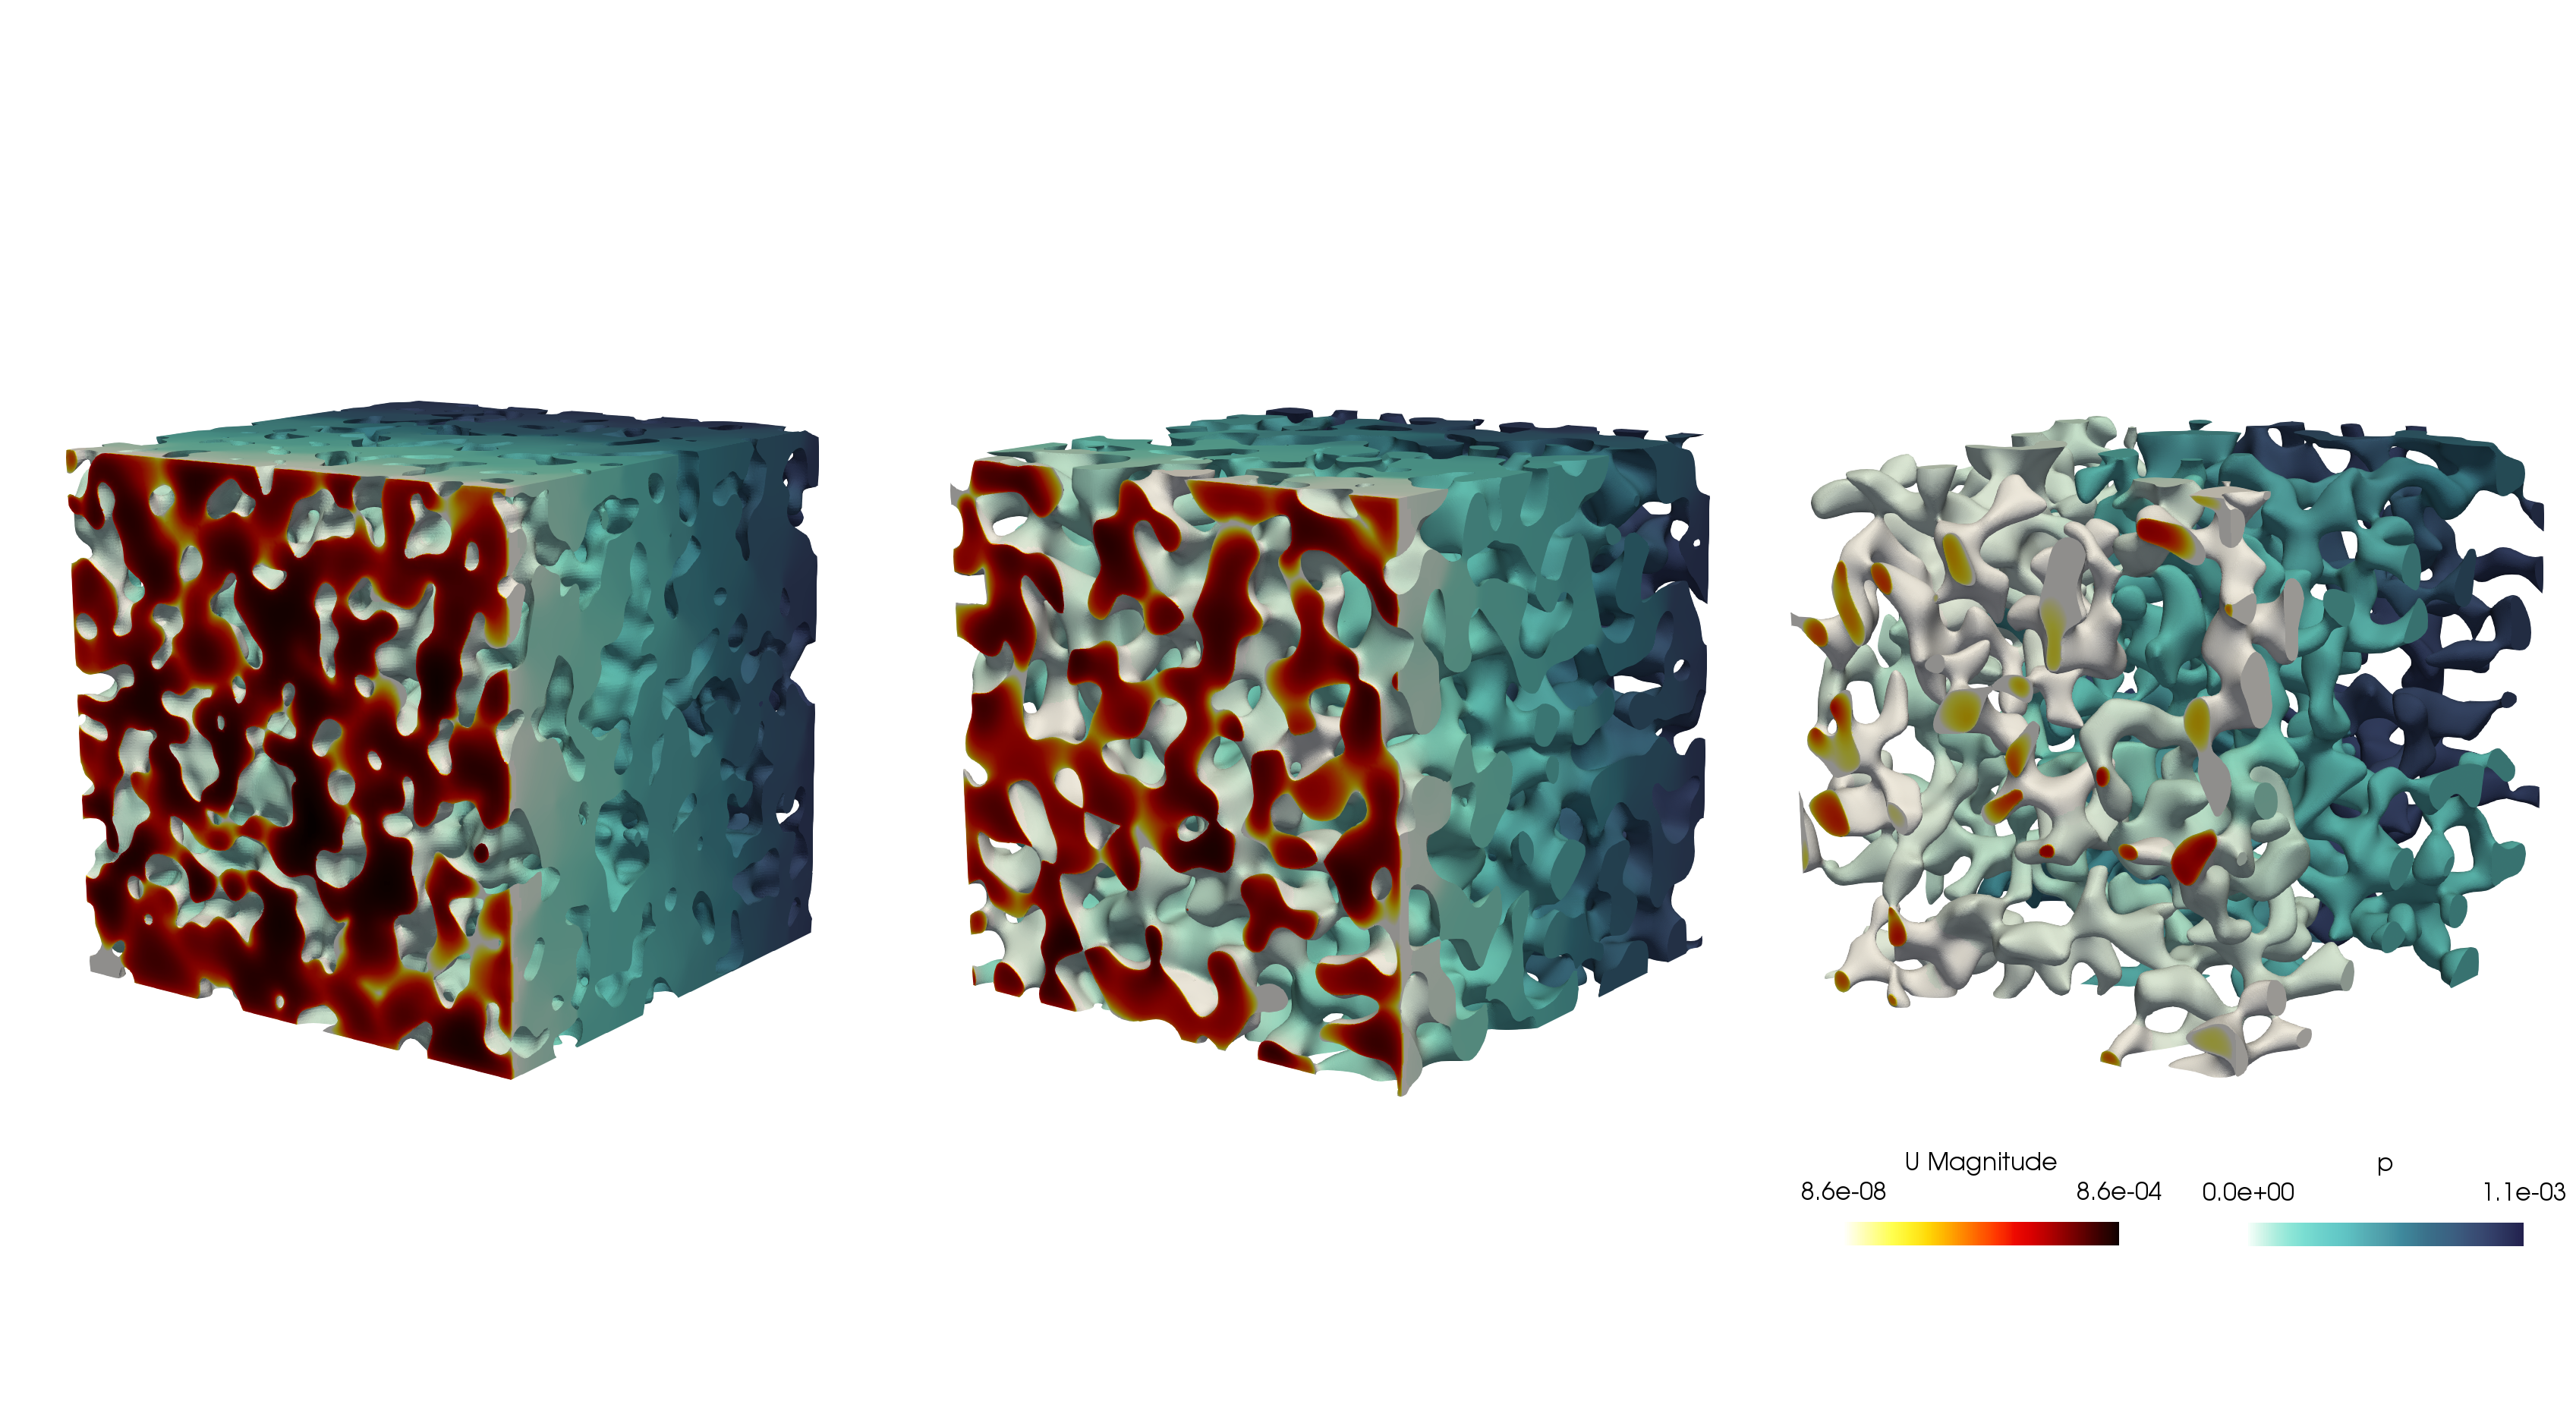
\includegraphics[height=8cm]{figures/PM_combined_surfaces_DNS.png}
\caption{A visualization of the velocity field $|u|$ and pressure field $p$ in the pore space of the three porous media used in this study.}
\label{fig:DNS}
\end{figure}


To generate heterogeneous porous media, that will form the basis for the direct numerical simulations, we have used Gaussian Random Fields to generate 3 porous media. A threshold is used to define the porous media-fluid interface $\Gamma$ and its porosity. In Table \ref{tab:results} we have collected the measures of these three porous media. The geometries are chosen such that we have a wide range in porosity $\phi$, relative pore size $l_p$ and surfaces roughness. The pore size is defined by $l_p = 4 \phi/s$ with $s= A_{\rm{tot}}/V$ the ratio of porous media interface $A_{\rm{tot}}$and the total volume $V$.The surface roughness is defined by the standard deviation of the mean curvature $H$ divided by the average pore size $l_p$. These measures are introduces to show the wide range of chosen geometries. These porous media are used as input for direct numerical simulations (OpenFOAM v. 4.1) \cite{weller_tensorial_1998} that solves the Navier-Stokes equations in the pore space. The boundary conditions are defined at the inlet $p_1$ and outlet $p_2$ and a no-slip for the porous media-fluid interface. A visualization of the three porous media is shown in Fig.~\ref{fig:DNS}. Then a chain of VTK-based image analysis techniques \citeA{schroeder_visualization_2006,hernderson_paraview_2007} are employed to extract iso-pressure surfaces $\mathcal{S}(p)$ and enumerate the disconnected areas identifying as an iso-pressure slice $\mathcal{S}_i(p)$, part of a pore and measure its surface area $A_i(p)$, sphericity $\gamma_i(p)$, average location $\mathbf{x}_i(p)$ and average flux $Q_i(p)$. For each $\mathcal{S}_i(p)$ its closest neighbor $\mathcal{S}_j(p+\delta p)$ is identified by its smallest distance $d_{i,j}= \left|  \mathbf{x}_i(p)-\mathbf{x}_j(p+\delta p)\right|$. By forward integration of the first iso-pressure patches $\mathcal{S}_i(p_0)$ we identify all patches belonging to the same pore $\mathcal{P}_l(\Delta p) = \{\mathcal{S}_k(p_i)\}$. Since the averaged coordinates of an iso-pressure surface is very sensitive to topological changes, a maximal distance between two consecutive coordinates can be used to define the end and the beginning of a pore. A visualization of such a topology change, or splitting and merging of pores is shown in Fig.\ref{fig:isop_surfaces} (Right). A description of chain of the VTK image analysis techniques is detailed in the SI. For each two consecutive iso-pressure surfaces that are part of a pore, we can now evaluate Eq.~\ref{eq:infi_dp} and for each pore, we can evaluate Eq.~\ref{eq:R_model}, and fit parameters $\alpha_i$ to obtain a model for the hydrualic resisistances for each porous media serperately. 


\section{Results}


The result of the DNS for the three porous media is shown in Fig.\ref{fig:DNS}. The obtained Reynolds number is estimated by $Re \sim l_p q/\nu$, with $q = Q/\overline{A}$. In figure \ref{fig:local_pressure_drop} the results of the infinitesimal pressure gradients (Eq.(\ref{eq:inf_dp})) are shown. We observe that the PH model underestimates the pressure gradient up to two orders of magnitude for the first porous media, to a relative good estimate for the third. The data is colored by the  sphericity, indicating the important role for the local hydraulic conductivity of a pore. The least scatter is found for the smallest pores For each porous media Eq.\ref{eq:infi_dp} has been fitted to obtain best estimates for $\alpha_i$ and listed in Table \ref{tab:results}. We observe that for the all porous media the sphericity is the most relevant parameter, and that the channelization parameter $\alpha_2$ is basically irrelevant.  The relative contributions of the $\alpha_0$ to $\alpha_1\gamma^{-2}$ is increasing with decreasing porosity in a similar manner. When the porosity is doubled the relative contribution of $\alpha_0$ is divided by two. For the third porous media we see that the relative contribution of sphericity is the smallest. This is to be expected since the pores are characterized with spericity close to 1 (see SI for a quantitative comparison). The Pearson correlation coefficients \citeA{}for these models are $0.93, 0.98, 0.99$ respectively. Because our data spans more orders of magnitude and the HP-model entails a high degree of heteroscedatisticy \citeA{white_heteroskedasticity-consistent_1980}, the Pearson correlation coefficient is not very reliable as a measure for the goodness of fit \citeA{wilcox_comparing_2009}. Therefore, we have chosen to list the ratio of the root-mean-squared error $\rm{RMSE}_m/\rm{RMSE}_{HP}$ in table \ref{tab:results}, showing a reduction of $\sim65\%$, as a measure for the goodness of the fits.  

\begin{figure}
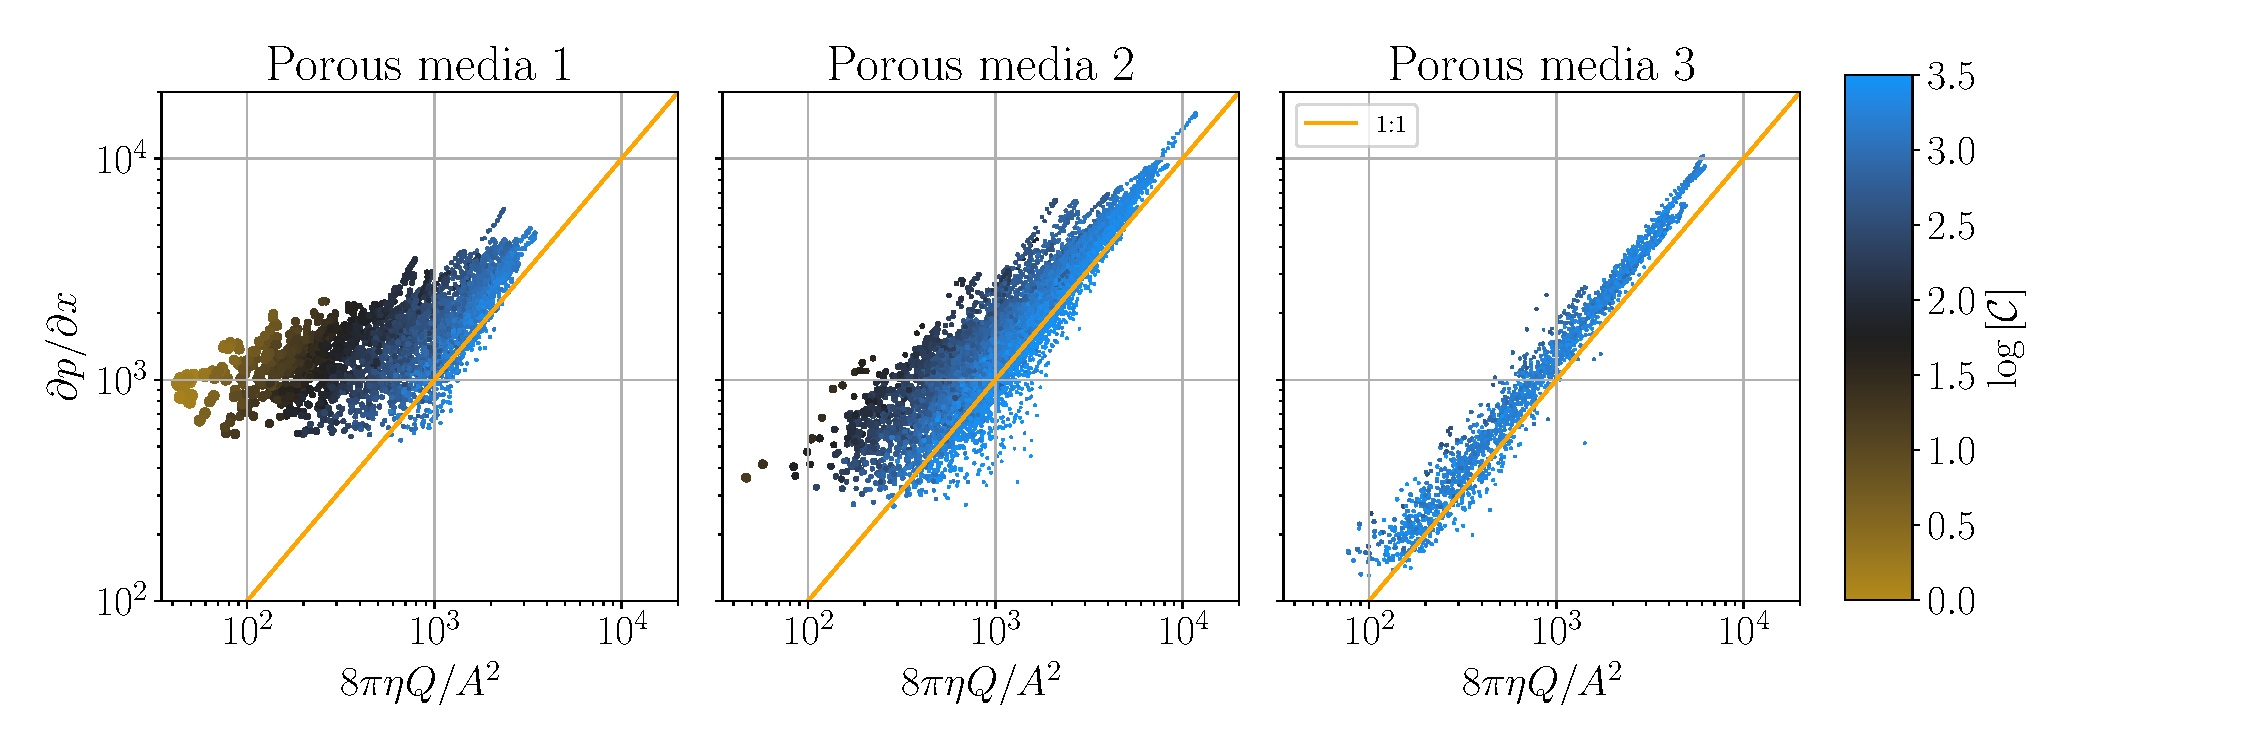
\includegraphics[height=6cm]{figures/infi_dpdx_3.pdf}
\caption{Measurements of local pressure drop versus the PH-model given by Eq.\ref{eq:HP} hydraulic resistance for three different porous media}
\label{fig:local_pressure_drop}
\end{figure}

\begin{figure}
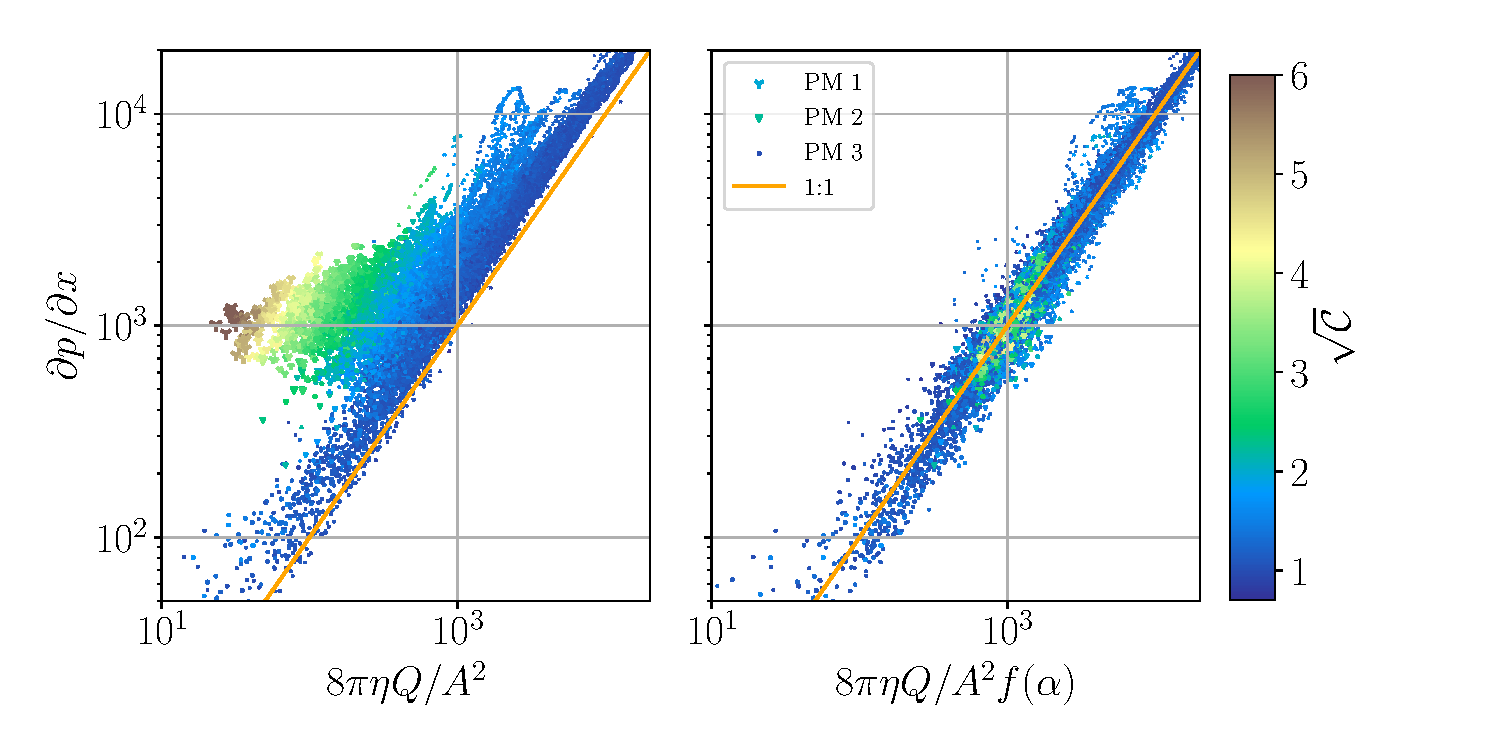
\includegraphics[height=8cm]{figures/infi_dpdx_combined.pdf}
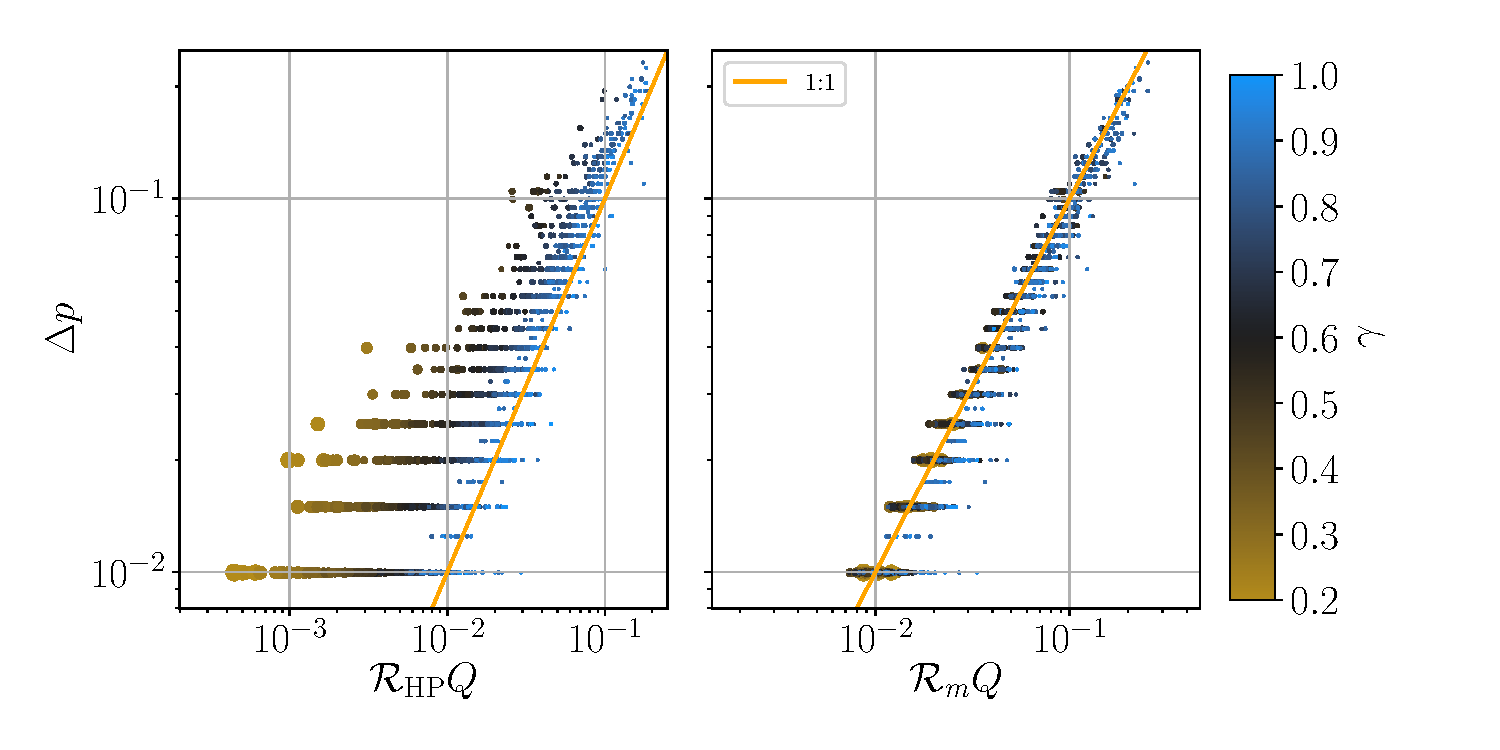
\includegraphics[height=8cm]{figures/integral_dp_combined.pdf}
\caption{Top Left: Measured infinitesimal pressure gradient versus the infinitesimal pressure drop of a Hagen-Poiseuille model, meaning $f(\alpha)\rightarrow 1$, for all three porous media combined. The relative cross-sectional area $A_i(p)$ is given by the markersize. Top Right: Measured versus Modeled infinitesimal pressure gradient with $f(\alpha)$ fitted to Eq.(\ref{eq:}) for each porous media separately. Bottom Left: Integrated pressure drop for extracted pores vs the HP-model for the hydraulic resistance $\mathcal{R}_{HP}$ times the total Flux $Q$ Bottom Right: Integrated pressure drop for extracted pores vs the modelled hydraulic resistance $\mathcal{R}_m$ (Eq.(\ref{eq:R_model})times the total Flux $Q$. The relative averaged pore cross-sectional area $A_i(p)$ is given by the markersize.}
\label{fig:local_and_integrated}
\end{figure}

Fitted values for


\begin{table}[htbp!]
\caption{Summary of the geometrical and fitting parameters}
\resizebox{\textwidth}{!}{
\centering
\begin{tabular}{l|c|c|c|c|c|c|c|c|c|c}
- & porosity & $A_{\rm{tot}}/V$ & $ l_p/L$ &  $\rm{std}(H)^{-1}/l_p$& $\alpha_0$, rel. & $\alpha_1$, rel. & $\alpha_2$, rel. & $\rm{RMSE}_m/\rm{RMSE}_{HP}$ & Re\\
\hline
PM1 &$0.68$ & $2.0\times10^{4}$ & $0.17$ &  $0.14$& $0.26,~14\%$ & $0.72,~86\%$ & $4.7\times 10^{-3}$ &  $0.32$&$\sim 10^{-2}$\\
PM2 & $0.34$ & $1.8\times10^{4}$ & $0.08$ &  $0.44$& $0.40,~29\%$ & $0.69,~71\%$ & $1.3 \times 10^{-3}$ & $0.42$&$\sim 10^{-2}$ \\
PM3 & $0.17$ & $1.2\times10^{4}$ & $0.06$ &  $0.35$& $0.98,~69\%$ & $0.32,~30\%$ & $0.22,~1\%$ & $0.34$&$\sim10^{-3}$ \\
\end{tabular}
\label{tab:results}
}
\end{table}





\section{Discussions}

Because the chosen method to extract pores from Openfoam data is new, it deserves a closer inspection that points out sensitivities and pitt-falls. 
The main issue with the data format of the OpenFoam simulations is that it is unstructured, and the meshing is refined towards the boundary of the porous media $\Gamma$. Although this ensures that the geometry is accurately described and that the simulation convergences, it also cause problems by extracting $\mathcal{S}(p)$ by a Contour function. Since it is based on a threshold it breaks up the mesh close to $\Gamma$ into many disconnected small area patches. To remove these small patches a threshold of a relatively low value for $\left|u\right|< \epsilon$ is chosen. This results in much smoother, but slightly smaller iso-pressure surfaces 

\begin{enumerate}

	\item Choosing $u_0$ to minimize point noise area patches of $S_i$, because of the mesh representation close to the interface.
	\item Choosing $dx_{max}$
	\item small pores, can also have a very complex shape, since there are more topology changes to be expected when $S_i$ is highly convoluted, as indicated by high $\gamma$. for Eq.~\ref{eq:infi_dp} needs at least 2 isopressure surface patches. 

	\item Channelization However, we found that only for porous media 3 that the Pearson correlation between $\alpha_0 +\alpha_1\gamma^{-2}$ and $\left|\frac{\partial A}{\partial x }\right|^2/A$ is $R^2= 0.25$, and can therefore be an indicator that channelization in the form of \ref{eq:tau_2} could still be relevant for pipe-like porous media. 

	\item sphericity values higher than $\gamma >0$



	\item Measured resistances function $f(\alpha) < 1$, is physically impossible. Here we measure a small portion that violates this physics. this is possible due to the method of cutting the iso pressure surfaces with a value $u_{min}$ leading to smaller areas. We have tried to correct for it with a factor that is calculated by the difference between the maximum $v_{max}-v_{min}$ by a linear extension of the area.  , but it is difficult to do this for very small areas since the cutoff of the area by $v_min$ is quit a significant portion. 
	\item The removal of the all the noise produced from the very fine mesh at close to the porous media interface is practically impossible, therefore, the final data has another threshold in the post processing on very small areas.   
	\item We can relax the condition of the boundary of a pore from $|u| = 0$ to $|u| < \epsilon$, reducing the complexity of the geometry of iso-pressure surfaces. The image analysis techniques become therefore much more complex and involve an analysis bases on the Morse-Smale Complex from the Topology ToolKit \cite{tierny_topology_2018} which is an extension of the VTK image analysis techniques used above. We have implemented this for the first porous media and found that the scatter in figure \ref{fig:local_pressure_drop} is significantly reduced. However when we fit the data to $f(\alpha_i)$, we find a similar, slightly worse performance of the model. This finding is relevant in two ways. The fist is that the order of magnitude of the local hydraulic resistance is well captured by the sphericity parameter, and this is valid even when the iso-pressure surfaces become very large, e.g. much larger than the average pore size. The second way is that iso-pressure surfaces can be subdivided into smaller pores which makes it easier to develop a method that extracts iso-pressure surfaces based on the geometry without doing the expensive actual DNS.  
\end{enumerate}


\subsection{Integrated along pores}

\begin{figure}
\centering{
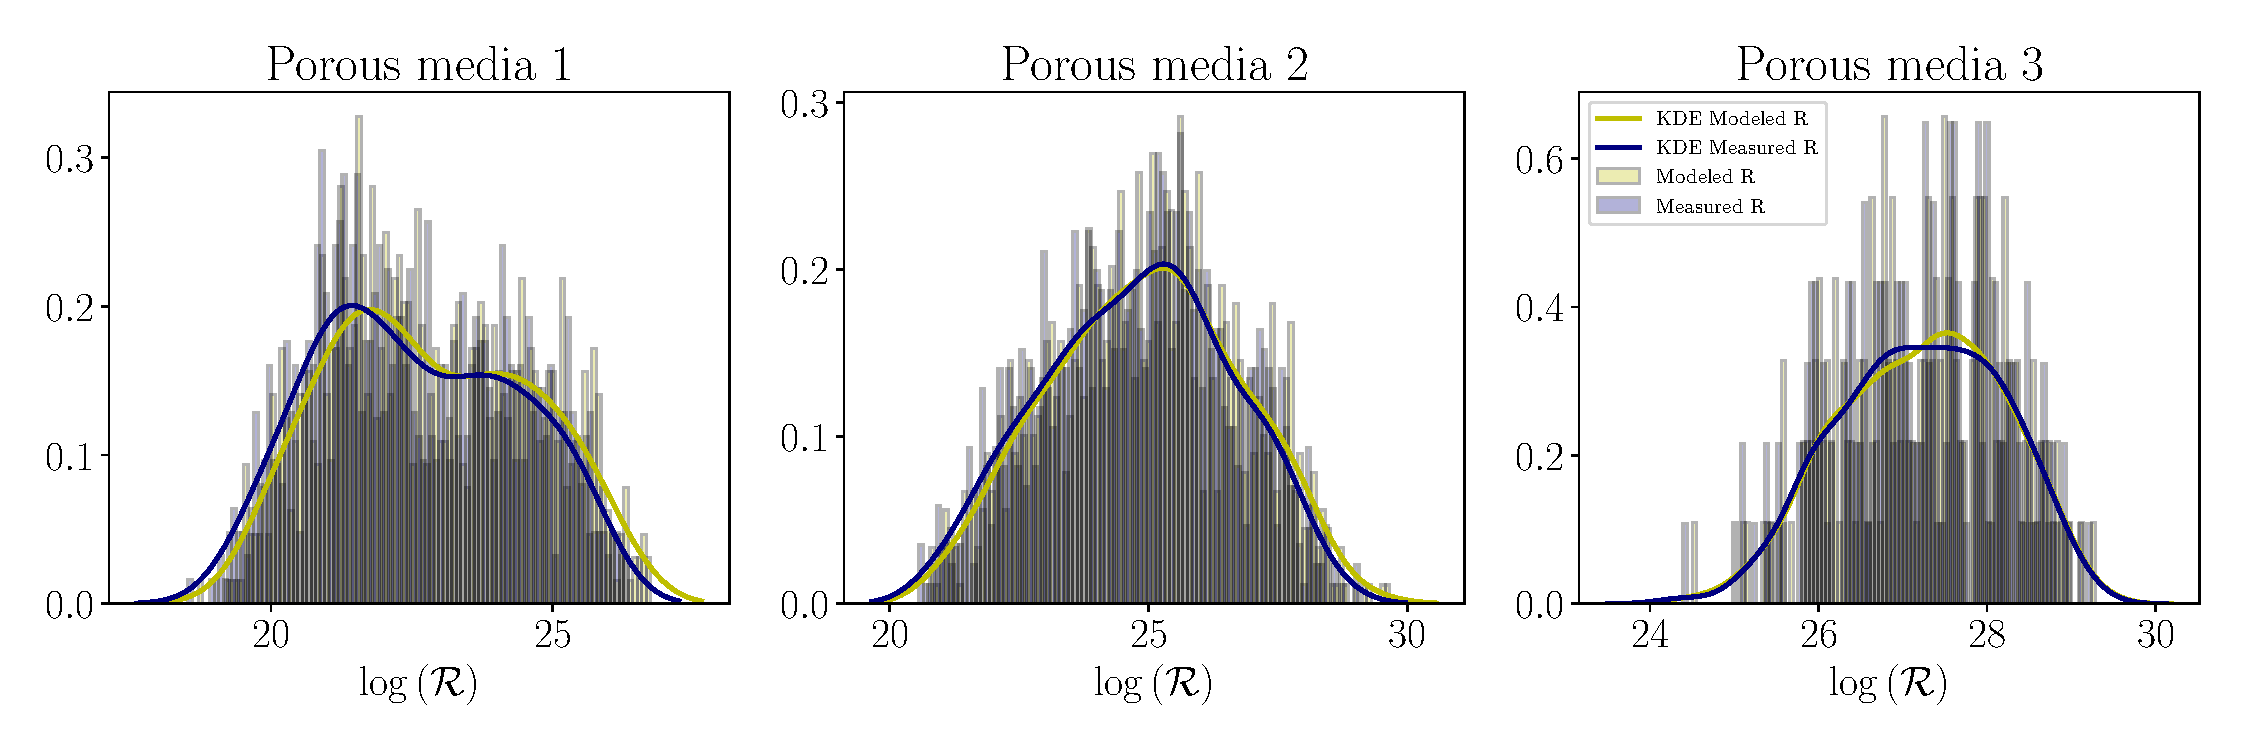
\includegraphics[height=5cm]{figures/hydraulic_conductivity_integrated_histogram.pdf}
\caption{Histogram of the measured and modeled hydraulic resistance $\mathcal{R}$.}}
\label{fig:histogram_R}
\end{figure}


\section{Odd observations}
\begin{itemize}
	\item $u_s$ is relatively high when iso-pressure surfaces have a hole, (genus < 0)
\end{itemize}

\section{Conclusions}
\begin{itemize}
	\item We have performed direct numerical simulations of laminar flow in three distinct heterogeneous porous media that vary in porosity and roughness.  
	\item We propose a new definition of individual pores in heterogeneous porous media with the aim of modeling the local hydraulic resistance that can be used in a pore-network model. The pores are defined a collection of disjoint iso-pressure surfaces that are topologically similar. If, by increasing or decreasing pressure, the topology of the iso-pressure surface changes the beginning and the end of the pore is defined. With this definition also the local flux $Q_i(p)$ remains constant throughout the pore. 
	\item We can measure the local hydraulic resistance by dividing the total pressure drop by the flux of the pore, and find that it can span approximately two orders of magnitude for the 3 porous media that we have analyzed. 
	\item The definition of the pores allows us to estimate the local hydraulic resistance in terms of the viscous dissipation tensor. This can be modeled by the sphericity of the iso-pressure surfaces and the channelization of the pore, that significantly improves on the Hagen-Poiseuille resistance of pipes. 
	\item One of the key observations of our work is the possibility of introducing a local geometric factor that provides for the ratio of pressure difference and mass flux in a given channel. The factor depends on the considered channel and not the rest of the complicated shape of the medium boundary. The non-triviality of this observation is made transparent by employing the boundary integral representation which is equivalent to the Stokes equations obeyed by the flow. The representation gives the flow as an integral over the medium surface where the points of the surface appear as sources that produce the flow as superposition. The ``charge" of such sources is proportional to the stress tensor at the boundary and the flow that each charge induces in space is given by an appropriate Green's function, see , see e.g. \cite{pozrikidis_boundary_1992}. Our result demonstrates that contributions other than those from the boundary of the considered channel can be neglected in the superposition. The mechanism by which this occurs consists of both screening effect and destructive interference between different channels. It needs further studies which are beyond our scope here.
\end{itemize}



%???? We observe that $dS_k=dS \nabla_k p/|\nabla p|$.


% \subsection{Hagen-Poiseuille Flow} 

% For a specific geometry of a pipe with Radius $R$ and length $L$, the second term from Eq.\ref{eq:pressuredrop} of the right-hand-side vanishes by symmetry considerations (i.e. the viscous work is zero). The exact solution for the local velocity can be obtained and is given by 
% \begin{equation}\label{eq:poiseuille}
% v(r)=U \left(1-\frac{r^2}{R^2}\right),
% \end{equation}
% with $U$ the maximal velocity. The flux $Q$, pressure gradient and the hydraulic resistance $\mathcal{R}:=\Delta p/Q$ can be simply written by
% \begin{equation}
% 	Q=\frac{\pi R^2 U}{2}\,,\,\frac{\Delta p}{L}=-\frac{4\eta U}{R^2}\, , \, \mathcal{R}_{\rm{hp}}= \frac{\eta L}{\pi^2 R^4}
% \end{equation}


%Text here ===>>>


%%

%  Numbered lines in equations:
%  To add line numbers to lines in equations,
%  \begin{linenomath*}
%  \begin{equation}
%  \end{equation}
%  \end{linenomath*}



%% Enter Figures and Tables near as possible to where they are first mentioned:
%
% DO NOT USE \psfrag or \subfigure commands.
%
% Figure captions go below the figure.
% Table titles go above tables;  other caption information
%  should be placed in last line of the table, using
% \multicolumn2l{$^a$ This is a table note.}
%
%----------------
% EXAMPLE FIGURES
%
% \begin{figure}
% \includegraphics{example.png}
% \caption{caption}
% \end{figure}
%
% Giving latex a width will help it to scale the figure properly. A simple trick is to use \textwidth. Try this if large figures run off the side of the page.
% \begin{figure}
% \noindent\includegraphics[width=\textwidth]{anothersample.png}
%\caption{caption}
%\label{pngfiguresample}
%\end{figure}
%
%
% If you get an error about an unknown bounding box, try specifying the width and height of the figure with the natwidth and natheight options. This is common when trying to add a PDF figure without pdflatex.
% \begin{figure}
% \noindent\includegraphics[natwidth=800px,natheight=600px]{samplefigure.pdf}
%\caption{caption}
%\label{pdffiguresample}
%\end{figure}
%
%
% PDFLatex does not seem to be able to process EPS figures. You may want to try the epstopdf package.
%

%
% ---------------
% EXAMPLE TABLE
%
% \begin{table}
% \caption{Time of the Transition Between Phase 1 and Phase 2$^{a}$}
% \centering
% \begin{tabular}{l c}
% \hline
%  Run  & Time (min)  \\
% \hline
%   $l1$  & 260   \\
%   $l2$  & 300   \\
%   $l3$  & 340   \\
%   $h1$  & 270   \\
%   $h2$  & 250   \\
%   $h3$  & 380   \\
%   $r1$  & 370   \\
%   $r2$  & 390   \\
% \hline
% \multicolumn{2}{l}{$^{a}$Footnote text here.}
% \end{tabular}
% \end{table}

%% SIDEWAYS FIGURE and TABLE
% AGU prefers the use of {sidewaystable} over {landscapetable} as it causes fewer problems.
%
% \begin{sidewaysfigure}
% \includegraphics[width=20pc]{figsamp}
% \caption{caption here}
% \label{newfig}
% \end{sidewaysfigure}
%
%  \begin{sidewaystable}
%  \caption{Caption here}
% \label{tab:signif_gap_clos}
%  \begin{tabular}{ccc}
% one&two&three\\
% four&five&six
%  \end{tabular}
%  \end{sidewaystable}

%% If using numbered lines, please surround equations with \begin{linenomath*}...\end{linenomath*}
%\begin{linenomath*}
%\begin{equation}
%y|{f} \sim g(m, \sigma),
%\end{equation}
%\end{linenomath*}

%%% End of body of article

%%%%%%%%%%%%%%%%%%%%%%%%%%%%%%%%
%% Optional Appendix goes here
%
% The \appendix command resets counters and redefines section heads
%
% After typing \appendix
%
%\section{Here Is Appendix Title}
% will show
% A: Here Is Appendix Title
%
%\appendix
%\section{Here is a sample appendix}

%%%%%%%%%%%%%%%%%%%%%%%%%%%%%%%%%%%%%%%%%%%%%%%%%%%%%%%%%%%%%%%%
%
% Optional Glossary, Notation or Acronym section goes here:
%
%%%%%%%%%%%%%%
% Glossary is only allowed in Reviews of Geophysics
%  \begin{glossary}
%  \term{Term}
%   Term Definition here
%  \term{Term}
%   Term Definition here
%  \term{Term}
%   Term Definition here
%  \end{glossary}

%
%%%%%%%%%%%%%%
% Acronyms
%   \begin{acronyms}
%   \acro{Acronym}
%   Definition here
%   \acro{EMOS}
%   Ensemble model output statistics
%   \acro{ECMWF}
%   Centre for Medium-Range Weather Forecasts
%   \end{acronyms}

%
%%%%%%%%%%%%%%
% Notation
%   \begin{notation}
%   \notation{$a+b$} Notation Definition here
%   \notation{$e=mc^2$}
%   Equation in German-born physicist Albert Einstein's theory of special
%  relativity that showed that the increased relativistic mass ($m$) of a
%  body comes from the energy of motion of the body—that is, its kinetic
%  energy ($E$)—divided by the speed of light squared ($c^2$).
%   \end{notation}




%%%%%%%%%%%%%%%%%%%%%%%%%%%%%%%%%%%%%%%%%%%%%%%%%%%%%%%%%%%%%%%%
%
%  ACKNOWLEDGMENTS
%
% The acknowledgments must list:
%
% >>>>	A statement that indicates to the reader where the data
% 	supporting the conclusions can be obtained (for example, in the
% 	references, tables, supporting information, and other databases).
%
% 	All funding sources related to this work from all authors
%
% 	Any real or perceived financial conflicts of interests for any
%	author
%
% 	Other affiliations for any author that may be perceived as
% 	having a conflict of interest with respect to the results of this
% 	paper.
%
%
% It is also the appropriate place to thank colleagues and other contributors.
% AGU does not normally allow dedications.


\acknowledgments
Enter acknowledgments, including your data availability statement, here.


%% ------------------------------------------------------------------------ %%
%% References and Citations

%%%%%%%%%%%%%%%%%%%%%%%%%%%%%%%%%%%%%%%%%%%%%%%
%
% \bibliography{<name of your .bib file>} don't specify the file extension
%
% don't specify bibliographystyle
%%%%%%%%%%%%%%%%%%%%%%%%%%%%%%%%%%%%%%%%%%%%%%%

\bibliography{library.bib}



%Reference citation instructions and examples:
%
% Please use ONLY \cite and \citeA for reference citations.
% \cite for parenthetical references
% ...as shown in recent studies (Simpson et al., 2019)
% \citeA for in-text citations
% ...Simpson et al. (2019) have shown...
%
%
%...as shown by \citeA{jskilby}.
%...as shown by \citeA{lewin76}, \citeA{carson86}, \citeA{bartoldy02}, and \citeA{rinaldi03}.
%...has been shown \cite{jskilbye}.
%...has been shown \cite{lewin76,carson86,bartoldy02,rinaldi03}.
%... \cite <i.e.>[]{lewin76,carson86,bartoldy02,rinaldi03}.
%...has been shown by \cite <e.g.,>[and others]{lewin76}.
%
% apacite uses < > for prenotes and [ ] for postnotes
% DO NOT use other cite commands (e.g., \citet, \citeA, \citeyear, \nocite, \citealp, etc.).
%



\end{document}



More Information and Advice:

%% ------------------------------------------------------------------------ %%
%
%  SECTION HEADS
%
%% ------------------------------------------------------------------------ %%

% Capitalize the first letter of each word (except for
% prepositions, conjunctions, and articles that are
% three or fewer letters).

% AGU follows standard outline style; therefore, there cannot be a section 1 without
% a section 2, or a section 2.3.1 without a section 2.3.2.
% Please make sure your section numbers are balanced.
% ---------------
% Level 1 head
%
% Use the \section{} command to identify level 1 heads;
% type the appropriate head wording between the curly
% brackets, as shown below.
%
%An example:
%\section{Level 1 Head: Introduction}
%
% ---------------
% Level 2 head
%
% Use the \subsection{} command to identify level 2 heads.
%An example:
%\subsection{Level 2 Head}
%
% ---------------
% Level 3 head
%
% Use the \subsubsection{} command to identify level 3 heads
%An example:
%\subsubsection{Level 3 Head}
%
%---------------
% Level 4 head
%
% Use the \subsubsubsection{} command to identify level 3 heads
% An example:
%\subsubsubsection{Level 4 Head} An example.
%
%% ------------------------------------------------------------------------ %%
%
%  IN-TEXT LISTS
%
%% ------------------------------------------------------------------------ %%
%
% Do not use bulleted lists; enumerated lists are okay.
% \begin{enumerate}
% \item
% \item
% \item
% \end{enumerate}
%
%% ------------------------------------------------------------------------ %%
%
%  EQUATIONS
%
%% ------------------------------------------------------------------------ %%

% Single-line equations are centered.
% Equation arrays will appear left-aligned.

% Math coded inside display math mode \[ ...\]
%  will not be numbered, e.g.,:
%  \[ x^2=y^2 + z^2\]

%  Math coded inside \begin{equation} and \end{equation} will
%  be automatically numbered, e.g.,:
%  \begin{equation}
%  x^2=y^2 + z^2
%  \end{equation}


% To create multiline equations, use the
% \begin{eqnarray} and \end{eqnarray} environment
% as demonstrated below.
% \begin{eqnarray}
%   x_{1} & = & (x - x_{0}) \cos \Theta \nonumber \\
%         && + (y - y_{0}) \sin \Theta  \nonumber \\
%   y_{1} & = & -(x - x_{0}) \sin \Theta \nonumber \\
%         && + (y - y_{0}) \cos \Theta.
% \end{eqnarray}

%If you don't want an equation number, use the star form:
%\begin{eqnarray*}...\end{eqnarray*}

% Break each line at a sign of operation
% (+, -, etc.) if possible, with the sign of operation
% on the new line.

% Indent second and subsequent lines to align with
% the first character following the equal sign on the
% first line.

% Use an \hspace{} command to insert horizontal space
% into your equation if necessary. Place an appropriate
% unit of measure between the curly braces, e.g.
% \hspace{1in}; you may have to experiment to achieve
% the correct amount of space.


%% ------------------------------------------------------------------------ %%
%
%  EQUATION NUMBERING: COUNTER
%
%% ------------------------------------------------------------------------ %%

% You may change equation numbering by resetting
% the equation counter or by explicitly numbering
% an equation.

% To explicitly number an equation, type \eqnum{}
% (with the desired number between the brackets)
% after the \begin{equation} or \begin{eqnarray}
% command.  The \eqnum{} command will affect only
% the equation it appears with; LaTeX will number
% any equations appearing later in the manuscript
% according to the equation counter.
%

% If you have a multiline equation that needs only
% one equation number, use a \nonumber command in
% front of the double backslashes (\\) as shown in
% the multiline equation above.

% If you are using line numbers, remember to surround
% equations with \begin{linenomath*}...\end{linenomath*}

%  To add line numbers to lines in equations:
%  \begin{linenomath*}
%  \begin{equation}
%  \end{equation}
%  \end{linenomath*}



